\documentclass[../../FisicaTeorica.tex]{subfiles}

\begin{document}

\begin{comment}
\section{Lezione X:\\ \large{Particelle indistinbuibili - parte 2}}
\vspace{-1em}
\begin{center}
    \small{(12/12/2018)}
\end{center}
\end{comment}

%Riporto qui l'ultima parte del 10/12
\section{Particelle identiche}
In \MC possiamo sempre \textbf{distinguere} due particelle \textbf{identiche}, dove per \textit{particelle identiche} intendiamo particelle che hanno le \textit{stesse proprietà indipendenti dallo stato} (stessa massa, carica, etc.).\\
Denotando con $q_t^{(j)}$ e $p_t^{(j)}$ posizione e momento al tempo $t$ della particella $j$-esima, consideriamo ad un certo $t_0$ il punto nello spazio delle fasi che descrive lo \textit{stato puro} del sistema. Se vale $(q_{t_0}^{(1)}, p_{t_0}^{(2)}) \neq (q_{t_0}^{(2)},p_{t_0}^{(2)})$, ossia se le due particelle sono \q{distinte} in almeno una tra posizione e momento, per l'unicità della soluzione delle equazioni del moto con condizioni iniziali date, le loro traiettorie nello spazio delle fasi non si intersecheranno mai nella loro evoluzione temporale.\\
\textit{In pratica, due particelle che sono identiche, es. due elettroni, possono essere \q{contrassegnate} dalla loro \q{storia}, ossia dal percorso che hanno compiuto nello spazio delle fasi. Ciò le rende, almeno in teoria, \textbf{distinguibili}, cioè in principio è possibile riferirsi nello specifico ad una di esse, individuandola senza ambiguità. Notiamo però che qui stiamo usando un'ipotesi forte: che la \q{storia} di ogni particella sia univocamente determinata}.\\
In \MQ, tuttavia, anche supposto che all'istante iniziale le due particelle identiche abbiano due funzioni d'onda $\psi^{(1)}$, $\psi^{(2)}$ con supporti spaziali disgiunti, che descrivono gli stati delle particelle $(1)$ e $(2)$, la loro evoluzione tramite Schr\"odinger in generale può portare ad una \textit{sovrapposizione} dei loro supporti, dopo la quale non c'è più modo di sapere, anche ammesso che i supporti ritornino disgiunti, a quale di essi corrispondano le particelle $(1)$ o $(2)$.
\begin{figure}[H]
\centering
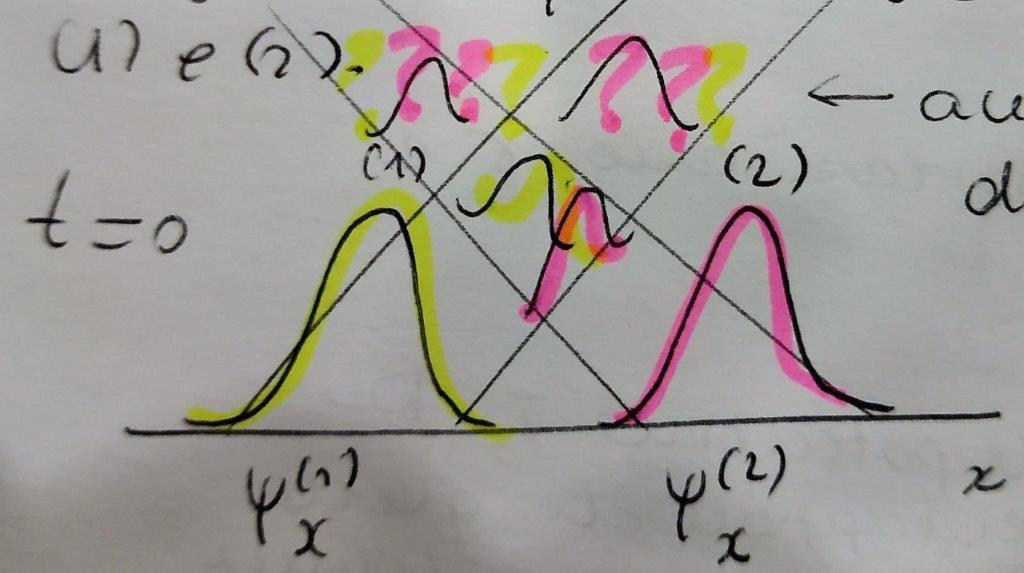
\includegraphics[scale=0.5]{Immagini/12_12/image001.jpg}
\caption{Dopo la sovrapposizione delle due funzioni d'onda (qui rappresentate come gaussiane) non è più possibile identificare esattamente a quale delle due particelle iniziali si riferiscano.}
\end{figure}
Graficamente, consideriamo due funzioni d'onda con supporto separato, che visualizziamo come due gaussiane che \textit{non si sovrappongono}. Vogliamo, ad ogni istante, dare un \textit{nome} alle due funzioni: se siamo in grado di farlo potremo considerare le due particelle \textit{distinguibili}. Ma se nella loro evoluzione le due funzioni si \textit{sovrappongono} e si separano di nuovo, non possiamo essere sicuri che la prima funzione abbia \q{rimbalzato} sulla seconda, oppure \q{le sia passata attraverso}. Abbiamo quindi una ambiguità sulla \textit{label} da assegnare alle funzioni d'onda.\\

Sperimentalmente, in un camera a nebbia, date le \q{traiettorie} di due particelle identiche che si intersecano (che sono in realtà costituite da un insieme finito di goccioline), non possiamo individuare \textit{quale \q{traiettoria} sia quella effettiva} dopo l'interazione.

\begin{figure}[H]
\centering
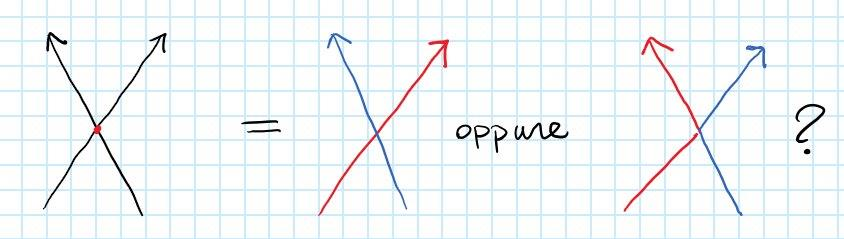
\includegraphics[scale=0.5]{Immagini/12_12/image002.jpg}
\caption{Ambiguità nel discernere la \q{traiettoria effettiva} partendo dai dati di \q{traiettoria} ottenuti da una camera a nebbia.}
\end{figure}

Perciò non esiste in linea di principio la possibilità di determinare una \textit{distinzione} tra particelle identiche a tutti gli istanti, ovvero non è possibile ancorare la loro individualità a caratteristiche estrinseche, dipendenti dallo stato (come la loro \q{storia} in senso classico).\\
Ciò ha una grossa conseguenza a livello fisico: ha infatti senso porsi \textbf{solo} domande che non dipendono dall'individualità delle particelle identiche, ad esempio la probabilità di trovare \textbf{un} elettrone in un fissato volume, ma non \textbf{un fissato} elettrone in quel volume.\\
Formalmente\marginpar{Conseguenza dell'indistinguibilità} ne segue che i \textbf{valori medi} di osservabili (sperimentalmente misurabili) in stati che differiscono per \textbf{scambio di particelle identiche} devono avere lo \textbf{stesso valore}.\\
Sappiamo che in \MQ lo spazio di Hilbert di $n$ particelle \textit{distinte} è il prodotto tensore degli spazi di ogni particella $\hs$. Quindi, se le $n$ particelle sono identiche, gli stati dovranno trovarsi tra i raggi vettori di $\hs^{\otimes \bb{N}} \equiv \hs \otimes \hs \otimes \dots \otimes \hs$.\\
Scelta una base $\{e_j\}_{j\in J}$ per $\hs$, sappiamo che $\{e_{j_1}\otimes e_{j_2} \otimes \dots \otimes e_{j_N}, j_i \in J\}$ è una base in $\hs^{\otimes \bb{N}}$.\\
Consideriamo le permutazioni di $N$ particelle identiche. Queste permutazioni costituiscono un gruppo\footnote{Dato che la composizione di permutazione è ancora una permutazione, per ogni permutazione esiste la \textit{permutazione inversa} che ne annulla l'azione, esiste la \q{permutazione nulla} che non modifica nessun ordine e vale la proprietà associativa per le permutazioni.}, denotato con $S_N$.\marginpar{Il gruppo $S_N$ delle permutazioni} Ogni elemento di $S_N$ rappresenta perciò un possibile \q{riordinamento} delle $N$ particelle. Intuitivamente, possiamo pensare ad ogni possibile permutazione come una serie di \textit{scambi} effettuati uno dopo l'altro. In effetti, si può dimostrare che semplicemente scambiando solo \q{elementi con i loro vicini} si può \textit{costruire} una permutazione generica.\\
Andando nello specifico, denotiamo con $1,2,\dots,N$ gli elementi su cui effettuiamo gli scambi e con $\sigma_i$ (che non ha nulla a che fare con le matrici di Pauli) l'operazione di scambio dell'elemento $i$-esimo con l'elemento $(i+1)$-esimo, dove $i = 0,\dots,N-1$. Si ha allora che una generica permutazione (elemento del gruppo $S_N$) si ottiene \textit{moltiplicando} delle $\sigma_i$, con i seguenti vincoli:
\begin{enumerate}
\item $\sigma_i^2 = 1$. In altre parole, scambiare due volte di fila le stesse particelle ($i$-esima e $(i+1)$-esima) non cambia nulla.
\begin{figure}[H]
\centering
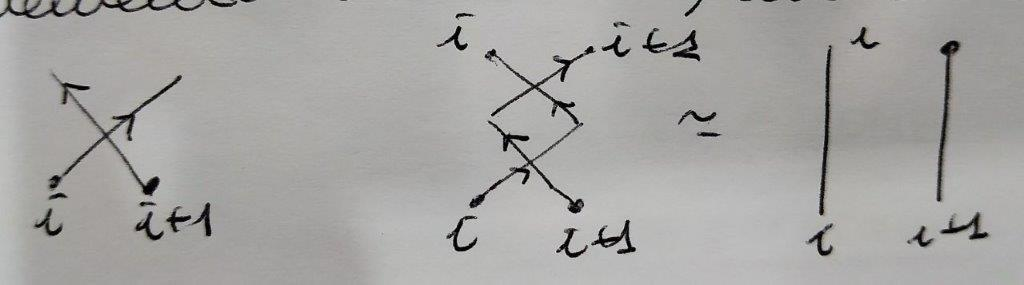
\includegraphics[scale=0.5]{Immagini/12_12/image003.jpg}
\caption{Illustrazione dell'effetto della permutazione $\sigma_i^2 = \op{id}$. L'idea del grafico sta nell'applicare le permutazioni \textit{una alla volta}, collegando ad ogni passo i punti \textit{di arrivo} di ciascuna particella con quelli \textit{di partenza}. Per esempio, dopo l'applicazione di una $\sigma_i$, la particella $i$ finisce nel posto $i+1$, e quella $i+1$ nel posto $i$. Una volta applicata la serie di permutazioni, si collega il punto di partenza di ogni particella con quello di arrivo finale, visualizzando così la \textit{permutazione risultante}.}
\end{figure}
\item $\sigma_i \sigma_j = \sigma_j \sigma_i$ se $|i-j|\geq 2$: due permutazioni di particelle \q{non contigue} sono indipendenti l'una dall'altra, e perciò non conta l'ordine in cui le si effettua. L'idea intuitiva è che ciascuna permutazione agisce \textit{localmente}, solo sull'$i$-esimo e $(i+1)$-esimo elemento, e perciò applicarle ad elementi che distano \q{più di un posto} uno dall'altro fa sì che non vi sia interazione tra le due.
\item $\sigma_i \sigma_{i+1}\sigma_i = \sigma_{i+1}\sigma_i\sigma_{i+1}$\\ %fare grafichetto [IMMAGINE]
Detto $A$ l'elemento di posto $i$-esimo, e $B$ e $C$ quelli di posti rispettivamente $i+1$ e $i+2$:
\begin{align*}
\sigma_i \sigma_{i+1}\sigma_i&:A\,B\,C\to B\,A\,C \to B\,C\,A \to C\,B\,A\\
\sigma_{i+1}\sigma_i \sigma_{i+1}&:
A\,B\,C \to A\,C\,B\to C\,A\,B \to C\,B\,A 
\end{align*}
Cioè scambiare prime due, poi seconde due e poi di nuovo prime due, oppure scambiare seconde due, poi prime due e poi di nuovo seconde due, produce la stessa cosa (ossia scambiare la prima con la terza).
\begin{figure}[H]
\centering
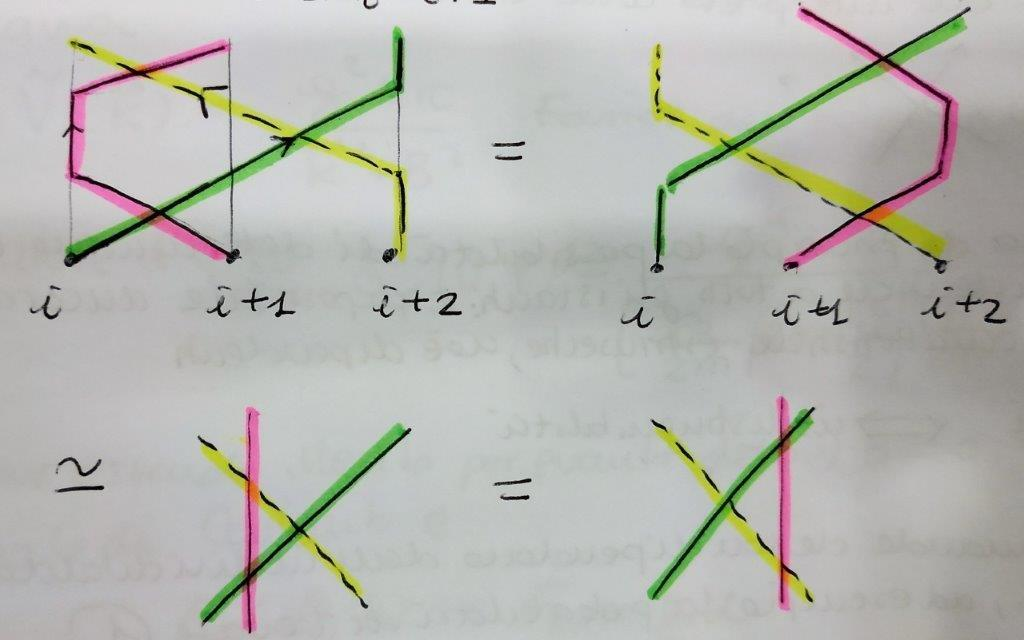
\includegraphics[scale=0.5]{Immagini/12_12/image004.jpg}
\caption{Graficamente, applichiamo in successione $\sigma_i$, $\sigma_{i+1}$ e $\sigma_i$ (figura a sinistra), oppure $\sigma_{i+1}$, $\sigma_i$ e $\sigma_{i+1}$ (figura a destra). Ad ogni passo colleghiamo con una linea (del colore della rispettiva particella) il \textit{punto di arrivo} con quello di \textit{partenza}: per esempio, nella figura in alto a destra il primo passo è $\sigma_{i+1}$, per cui la particella $i+1$ finisce al posto $i+2$, e quella $i+2$ al posto $i+1$, mentre quella $i$ rimane in $i$. Una volta eseguiti tutti i passi, colleghiamo punti di arrivo all'ultimo passo con quelli di partenza delle rispettive particelle al primo: notiamo che l'ordine (dei colori) è lo stesso sia nella figura a sinistra che in quella a destra - e ciò dimostra l'equivalenza che cercavamo.}
\end{figure}
\end{enumerate}
Le $\sigma_i$ così viste sono tuttavia \q{operazioni astratte}, e se vogliamo applicarle ai problemi che ci interessano dovremo sceglierne una \textit{rappresentazione} (analogamente a quanto già fatto per traslazioni e rotazioni).\\
Per ogni $\sigma\in S_N$ definiamo allora l'operatore unitario:
\begin{align*}
U(\sigma): e_{j_1}\otimes e_{j_2}\otimes \dots \otimes e_{j_N} \mapsto e_{\sigma(j_1)} \otimes e_{\sigma(j_2)} \otimes \dots \otimes e_{\sigma(j_N)}
\end{align*}
esteso per linearità e continuità a $\hs^{\otimes \bb{N}}$.\\
Nella notazione $\sigma(x)$ rappresenta il vettore che prende il posto di $x$ \textit{dopo} aver effettuato la permutazione. In altre parole $U(\sigma)$ \textit{scambia} tra loro le basi dei singoli $\hs$ che costituiscono $\hs^{\otimes\bb{N}}$, e costituisce quindi una rappresentazione unitaria di $S_N$ in $\hs^{\otimes \bb{N}}$ (ossia una \q{concretizzazione} della nozione astratta di permutazione).\\
Poiché vogliamo che i valori medi \textit{non} dipendano dalla permutazione, deve valere, $\forall \ket{\psi}\in \hs^{\otimes \bb{N}}$ e $\forall$ osservabile $A$ in $\hs^{\otimes \bb{N}}$ la condizione di \textbf{invarianza dei valor medi}:
\begin{align}
\bra{\psi} U^\dag(\sigma)AU(\sigma)\ket{\psi} =\ \bra{\psi}A\ket{\psi}\quad \forall \sigma \in S_N \Rightarrow U^\dag(\sigma)AU(\sigma)=A
\label{eqn:condizione-simmetria-scambi}
\end{align}
Perciò non tutti gli operatori autoaggiunti in\ $\hs^{\otimes \bb{N}}$ sono osservabili, ma solo quelli per cui vale (\ref{eqn:condizione-simmetria-scambi}). Poiché ogni operatore in $\hs^{\otimes \bb{N}}$ può scriversi come combinazione lineare (eventualmente infinita) di operatori $A_1 \otimes A_2 \otimes \dots \otimes A_N$, ove gli $A_i$, detti operatori di particella singola, agiscono sulla $i$-esima coppia di $\hs$ in $\hs^{\otimes \bb{N}}$, La (\ref{eqn:condizione-simmetria-scambi}) ci dice che \textbf{sono osservabili solo operatori autoaggiunti} in $\hs^{\otimes \bb{N}}$ \textbf{simmetrici} per \textit{ogni} scambio degli operatori di particella singola. In altre parole, per un sistema di $N$ particelle identiche, calcolare il valore di $A$ per la particella $i$-esima deve dare lo \textit{stesso} risultato per ogni $i$, dato che se le particelle sono indistinguibili non vi è un modo univoco di identificare la particella $i$ in questione.\\

Analogamente avremo una condizione di \textit{invarianza degli stati}, per cui \q{scambiare gli stati di due particelle identiche non cambia lo stato del sistema}, ossia $U(\sigma)\ket{\psi}$, $\forall \sigma \in S_N$, $\ket{\psi} \in \hs^{\otimes \bb{N}}$ deve descrivere lo stesso stato di $\ket{\psi}$. Poiché le $\sigma$ si possono scrivere come prodotti di $\sigma_i$, ci basta esaminare quest'ultimo caso.\\
Matematicamente, si ha che $U(\sigma_i)\ket{\psi}$ è pari a $\ket{\psi}$ a meno di un fattore moltiplicativo $c(\sigma_i)$:
\begin{align*}
U(\sigma_i)\ket{\psi} = c(\sigma_i)\ket{\psi}
\end{align*}
Per trovare $c(\sigma_i)$ ricordiamo la proprietà di \q{compatibilità per l'operazione di gruppo} per le rappresentazioni, ossia:
\begin{align*}
\sigma = \sigma_i \sigma_j \Rightarrow U(\sigma) = U(\sigma_i)U(\sigma_j)
\end{align*}
Applicando allora due volte di fila la stessa permutazione $\sigma_i^2$, sappiamo che il sistema rimane invariato ($\sigma_i^2 = e$, dove $e$ è l'elemento neutro di $S_N$). Perciò, usando la rappresentazione unitaria di $S_N$:
\begin{align*}
U(\sigma_i^2) =\ U(\sigma_i)U(\sigma_i)=U(\sigma_i)^2
\end{align*}
Inoltre, sempre dalla definizione di rappresentazione, $U$ manda l'elemento neutro $e$ nell'elemento neutro delle matrici, ossia $\bb{I}$:
\begin{align*}
U(\sigma_i^2) = U(e) = \bb{I}
\end{align*}
Applicando ad una generica $\ket{\psi}$ (normalizzata) otteniamo:
\begin{align*}
U(\sigma_i)^2 \ket{\psi} = c(\sigma_i)^2 \ket{\psi} = U(e)\ket{\psi} =\ket{\psi} \Rightarrow c(\sigma_i)^2 =1
\end{align*}

Prendendo la radice quadrata troviamo due possibilità: $c(\sigma_i)=\pm 1$.\\
Perciò, $\forall \sigma_i$ deve succedere:
\begin{itemize}
\item $c(\sigma_i) = 1$, ossia la funzione d'onda/il vettore di stato sono \textit{simmetrici per scambi} (non cambiano di segno dopo una permutazione). Le particelle che soddisfano questa condizione sono detti \textbf{bosoni}.
\item $c(\sigma_i)=-1$, dove invece funzione d'onda/vettore di stato sono \textit{antisimmetrici per scambi}. Le particelle che soddisfano quiesta proprietà sono i \textbf{fermioni}.
\end{itemize}

Tutto ciò porta a un fenomeno nuovo: i \textbf{settori di superselezione}\marginpar{Settori di superselezione}\index{Settori di superselezione}.\\
Poiché le osservabili sono \textit{simmetriche per scambi}, i sottospazi di $\hs^{\otimes \bb{N}}$ sede delle rappresentazioni simmetriche (bosoni) o antisimmetriche (fermioni) sono lasciati invariati dalle operazioni di evoluzione temporale e di misura. Infatti, il primo caso si realizza applicando l'esponenziale di un'osservabile -- $H$ -- che è simmetrica, mentre il secondo è dato dall'uso di proiettori, che essendo osservabili sono simmetrici.\\
Quindi gli stati simmetrici e antisimmetrici non si mescolano mai, qualsiasi operazione si faccia. Descrivono quindi \q{mondi distinti}, che tecnicamente si chiamano \textbf{settori di superselezione}\index{Settori di superselezione}.

\textit{Un altro esempio, meno ovvio, di settore di superselezione è dato dalla carica elettrica. Non è possibile sovrapporre due stati di carica diversa, e qualsiasi operazione si faccia non è possibile cambiarla. Operatori che non rispettano tali condizioni non costituiscono osservabili.}\\

Denotati con $\ket{\psi_i}$, $i=1, \dots, N$ i ket delle singole particelle identiche che compongono il sistema, sappiamo perciò che lo stato \q{totale} $\ket{\Psi}$ del sistema deve essere simmetrico o antisimmetrico per scambi di particelle, a seconda che esse siano rispettivamente bosoni o fermioni. In generale, il prodotto tensore delle $\ket{\psi_i}$ \textit{non} ha questa proprietà, e perciò dovremo considerare un'operazione più specifica: il prodotto tensore (anti)simmetrico.\\
L'idea è di combinare le $\ket{\psi_i}$ in modo che il risultante tensore sia (anti)simmetrico\footnote{Un'operazione analoga è definita formalmente nella lezione $10\_1$ nelle dispense del corso di \q{Geometria Differenziale} tenuto dal professor Bottacin.}. Per farlo basta sommare su \textit{tutte le permutazioni possibili} dei prodotti tensori delle $\ket{\psi_i}$ (eventualmente introducendo un fattore alternante): in questo modo l'effetto di una permutazione è quello di \textit{scambiare} due termini di una somma, lasciando invariato il risultato (a meno del segno, nel caso sia presente il fattore alternante). Esplicitamente, avremo le seguenti espressioni per $\ket{\Psi}$:
\begin{align*}
\ket{\Psi} &=\ \frac{1}{\sqrt{N!}}\sum_{\sigma \in S_N} \prod_i \ket{\psi_{\sigma(i)}} && \text{ket per $N$ bosoni}\\
\ket{\Psi} &= \frac{1}{\sqrt{N!}}\sum_{\sigma \in S_N} (-1)^{|\sigma|}\prod_i \ket{\psi_{\sigma(i)}} && \text{ket per $N$ fermioni}
\end{align*}
Dove con $|\sigma|$ indichiamo il numero di scambi effettuati per formare la permutazione $\sigma$ (che a priori non è ben definito, ma è ben definita la sua \textit{parità}, che è l'unica cosa che ci interessa nella formula di sopra).\\
Notiamo che tali stati per il sistema composto \textbf{non} sono il semplice prodotto tensore di ket di particelle singole $\ket{\psi_i}$, ma combinazioni lineari di tali prodotti, cioè sono \q{entangled}. Questa è la conseguenza \textit{fisica} della \textit{perdita dell'individualità}: il fatto che non si possa discutere di particelle singole (poiché non è possibile identificarle), fa sì che l'unico modo di descrivere il sistema sia in una \q{visione globale} che non può essere spezzata nelle singole parti.\\

\subsection{Il principio di esclusione di Pauli}
Una conseguenza immediata dell'antisimmetria per i fermioni è il seguente principio:\index{Principio di esclusione di Pauli}
\begin{thm}
\marginpar{Principio di esclusione di Pauli}\index{Principio di esclusione di Pauli}
Non è possibile per un sistema di $N$ fermioni identici avere due particelle con lo stesso insieme di autovalori di un ICOC.
\end{thm}
Ad esempio, consideriamo come $\hs$ lo spazio di Hilbert di particella singola per un atomo di idrogeno. Un ICOC è $\{H, \vec{L^2}, L_z, S_z\}$. Indichiamo i rispettivi autovalori di tali osservabili con $\{n, l, m, s_z\}$.\\
Per il principio di esclusione si ha che è impossibile mettere due elettroni con gli stessi $n, l, m, s_z$ nell'atomo di idrogeno - cioè al massimo vi sono due elettroni per \textit{orbitale} (dove un orbitale è definito da i numeri quantici $n,l,m$).\\
Lo stesso ICOC vale anche per un qualsiasi sistema coulombiano - e in particolare per atomi più complessi. In particolare, in un atomo con molti elettroni siamo costretti a mettere elettroni in orbitali a energia crescente per rispettare il principio di Pauli, e da ciò deriva tutta la \textit{chimica}.\\
In modo analogo, applicando il principio di esclusione di Pauli all'ICOC $\{\vec{X}, S_z\}$, risulta che (in modo \q{immaginifico}) due elettroni non possono avere neppure \q{potenzialmente} stessa posizione e spin.\\
Verifichiamolo. Ipotizziamo per assurdo che $\vec{x}_i, s_{z_i} = \vec{x_j}, s_{z_j}$, ossia che gli elettroni $i$-esimo e $j$-esimo abbiano stessa posizione e spin. Se partiamo da una funzione d'onda:
$\psi(\vec{x}_1, s_{z_1}, \dots, \vec{x}_N, s_{z_N})$
e scambiamo i due elettroni $i$ e $j$, sappiamo che il segno deve cambiare per l'antisimmetria (essendo gli elettroni fermioni):
\begin{align*}
&\psi(\vec{x}_1, s_{z_1}, \dots, \hlc{Yellow}{\vec{x}_i, s_{z_i}}, \dots \hlc{SkyBlue}{\vec{x}_j, s_{z_j}}, \dots, \vec{x}_N, s_{z_N})=\\
&=-
\psi(\vec{x}_1, s_{z_1}, \dots, \hlc{SkyBlue}{\vec{x}_j, s_{z_j}}, \dots \hlc{Yellow}{\vec{x}_i, s_{z_i}}, \dots, \vec{x}_N, s_{z_N})
\end{align*}
Ma se i due termini scambiati sono uguali (per ipotesi), allora le due $\psi$ devono essere uguali (scambiare gli stessi termini \textit{non} modifica la $\psi$). Ma allora l'unica possibilità per cui contemporaneamente $\psi=-\psi$ e $\psi=\psi$ è che sia $\psi=0$.\\
Poiché la funzione d'onda descrive le probabilità di misura, anche prima che essa venga effettuata, si ha che \textit{anche prima di una misura} gli elettroni non possono occupare gli stessi stati di posizione-spin.\\

Qualitativamente\marginpar{L'incompenetrabilità della materia} tale fenomeno spiega l'\textit{incompenetrabilità} della materia.\\
Esaminando la struttura atomica, infatti, non risulta per nulla evidente ad un primo sguardo perché due atomi non possano \q{attraversarsi}. Il nucleo è infatti incredibilmente piccolo rispetto alle distanze a cui \q{orbitano} gli elettroni -- per cui l'atomo è considerabile come quasi interamente \q{vuoto}, e anche la probabilità di un'interazione elettromagnetica significativa tra due $e^-$ è relativamente bassa.\\
Tuttavia, si ha che la sola \textit{potenzialità} di occupazione degli stessi stati è impedita dal principio di esclusione -- e perciò due atomi sono \textit{costretti} a rimanere ben separati, dato che la probabilità di \q{attraversarsi} è \textbf{nulla}.\\

Il principio di esclusione\marginpar{Le stelle di neutroni} è utile per comprendere anche la struttura delle \textbf{stelle di neutroni}. Se la forza di gravitazionale è sufficientemente intensa, gli orbitali sono \q{schiacciati} uno contro l'altro, ma non possono compenentrarsi per principio di esclusione. Tali condizioni favoriscono allora un processo che altrimenti è molto raro: un protone e un elettrone si \textit{fondono} a formare un neutrone (liberando un neutrino elettronico).
\begin{align*}
p^+ + e^- \to n + \nu_e
\end{align*}
I neutroni così prodotti possono ora \q{compattarsi} molto di più, dato che la distanza tra ciascuno di essi è dell'ordine di $10^{-15}m$. Ciò permetterebbe all'intera massa del Sole, che normalmente ha un raggio $\sim 700\cdot 10^3$km, di essere concentrata in un raggio di $10$km. La densità della materia \textit{degenere} così prodotta (detta \q{neutronio}) è tale che un solo $cm^3$ abbia una massa dell'ordine $\sim 2\cdot 10^6$kg.\\

\subsection{Effetti in dimensioni inferiori}
C'è un modo lievemente diverso di vedere la statistica (comportamento per scambi) che è rilevante in $d<3$ (trascuriamo, per ora, lo spin).\\
Consideriamo lo scambio di posizione di due particelle $x_i$ e $x_j$. Fisicamente possiamo pensarlo come un \textit{cammino continuo} che porta $x_i \to x_j$ e $x_j \to x_i$. Ci chiediamo: conta \textit{l'ordine} dello scambio? Se permutiamo $x_i$ e $x_j$ \q{in senso orario} otteniamo lo stesso risultato che nel caso \q{antiorario}?\\
In $d=3$, i due \textit{modi} di effettuare lo scambio sono equivalenti, dato che i due spostamenti possono avvenire contemporaneamente lungo curve che non si intersecano, come visibile in figura \ref{fig:scambio3d}.
\begin{figure}[H]
\centering
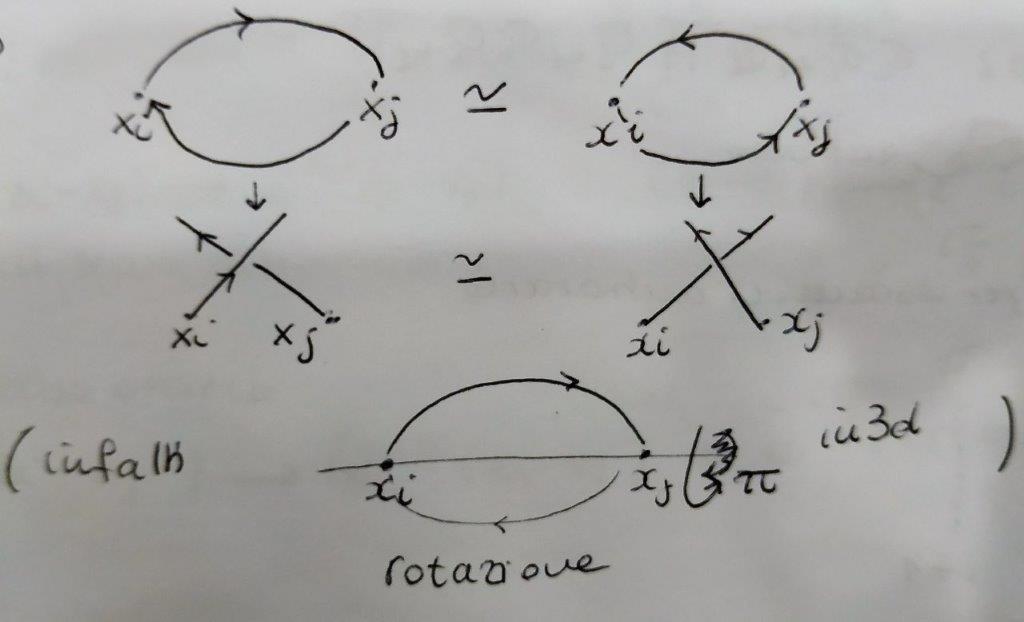
\includegraphics[scale=0.3]{Immagini/12_12/image005.jpg}
\caption{Scambio di $x_i$ e $x_j$ in $d=3$: possiamo immaginare di far passare $x_i$ \textit{sopra} al piano e $x_j$ \textit{sotto}, e in tal modo i due percorsi di scambio non si intersecano, e perciò l'ordine di scambio non conta: possiamo vedere una delle due possibilità (es. $x_i$ che passa sopra e $x_j$ sotto) come la versione \textit{ruotata} di $\pi$ dell'altra possibilità ($x_i$ sotto e $x_j$ sopra).\label{fig:scambio3d}}
\end{figure}
Per far ciò, tuttavia, abbiamo dovuto usare \textit{la terza dimensione spaziale}. Lo stesso trucco non funziona più in $d=2$, dove i cammini devono per forza intersecarsi, come visibile in figura \ref{fig:scambio2d}.
\begin{figure}[H]
\centering
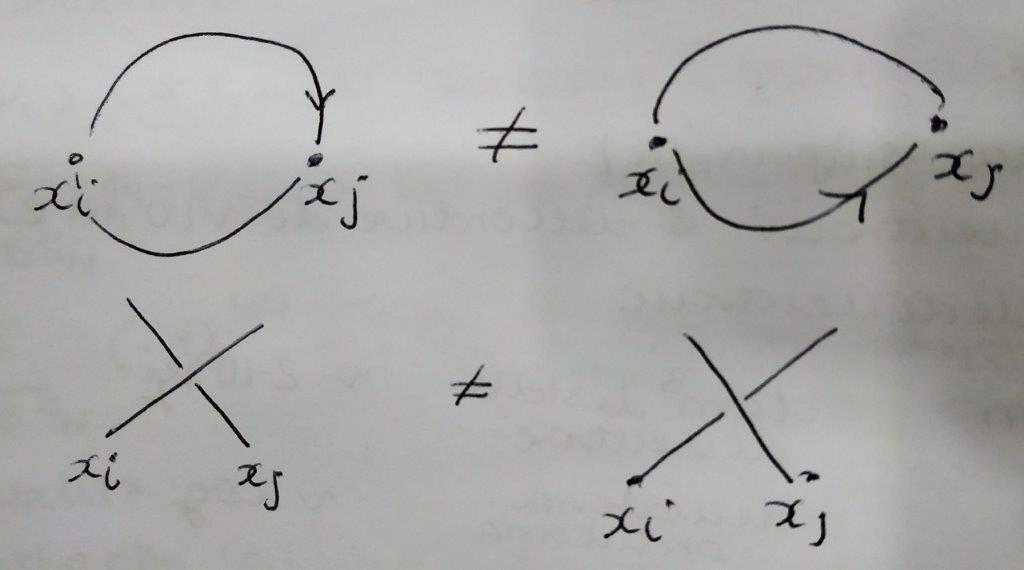
\includegraphics[scale=0.3]{Immagini/12_12/image006.jpg}
\caption{In $d=2$ i due percorsi si intersecano, e non c'è modo di convertire una scelta di ordine nell'altra.\label{fig:scambio2d}}
\end{figure}

Infatti, poiché stiamo considerando fermioni, le due particelle non possono occupare la stessa posizione allo stesso tempo. Avremo allora due possibilità \textit{non equivalenti}: uno scambio \textit{orario} e uno \textit{antiorario}. Non c'è modo di mappare uno nell'altro senza intersecare i cammini -- cosa che è proibita dalla natura fermionica delle particelle.\\
Una conseguenza di ciò è che avremo due tipi di \textit{permutazione} che scambiano gli elementi $i$-esimo e $i+1$-esimo: quella oraria $\sigma_i$ e quella antioraria $\sigma_{i}^{-1}$, con:
\begin{align*}
\sigma_i \neq \sigma_{i}^{-1} \qquad d=2
\end{align*}      
Una conseguenza immediata è che $\sigma_i^2\neq 1$: due permutazioni orarie consecutive \textit{non} riportano allo stato iniziale.\\
Possiamo visualizzare ciò in modo pittoresco, schematizzando il cammino di ogni particella durante la permutazione come un \textit{filo colorato}, come rappresentato in figura \ref{fig:braids}.

\begin{figure}[H]
\centering
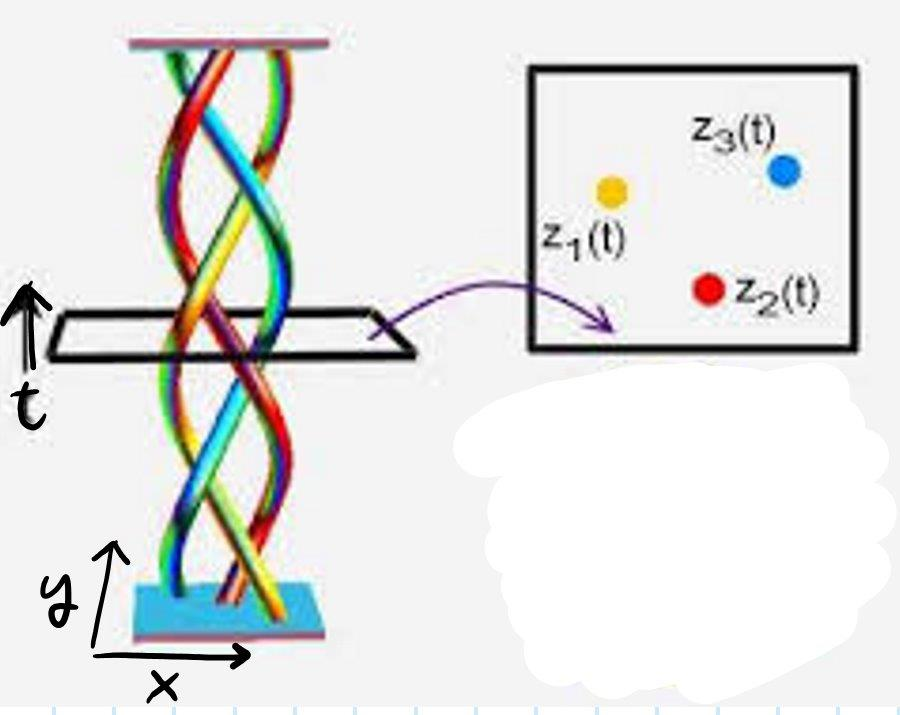
\includegraphics[scale=0.3]{Immagini/12_12/image007.jpg}
\caption{Schema dei cammini di $3$ particelle durante una permutazione\label{fig:braids}}
\end{figure}

In tale rappresentazione, scambiare due volte \textit{nello stesso senso} (es. orario) due particelle, fa sì che i loro cammini \textit{si intreccino}. Poiché non si può far passare un filo attraverso un altro (essendo le particelle fermioni), non è possibile \textit{separare} i due cammini dopo i due scambi orari, che quindi sono \textit{topologicamente} distinti dai due cammini \q{paralleli} (e non intrecciati) che avremmo avuto nel caso senza alcuna permutazione.\\
D'altro canto, applicare prima uno scambio orario e poi uno antiorario \textit{riporta} effettivamente alla situazione iniziale, dato che l'intreccio dato dalla prima operazione è \q{sciolto} dalla seconda.

\begin{figure}[H]
\centering
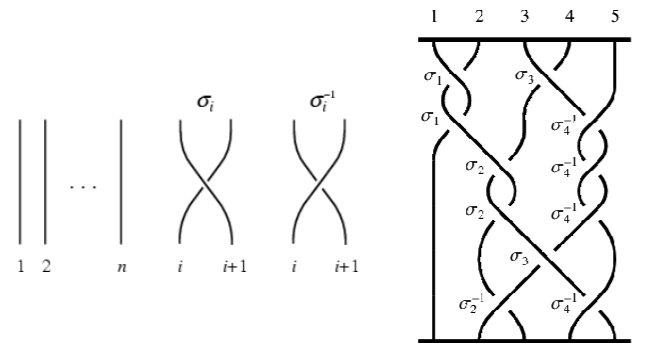
\includegraphics[scale=0.5]{Immagini/12_12/image008.jpg}
\caption{Esempio di intrecci generati dall'applicazione consecutiva di più permutazioni $\sigma_j$}
\end{figure}
%\footnote{Immagine tratta da \url{http://semana.mat.uson.mx/MemoriasXVII/XVII/21MiguelAXico.pdf}

Tutto ciò fa sì che non si possa più usare il gruppo $S_N$ per descrivere l'indistinguibilità di particelle in $d=2$. Al suo posto introduciamo il gruppo generato da prodotti di scambi \textit{con orientazione}, detto \textbf{gruppo delle trecce} $B_N$ per $N$ oggetti\footnote{La $B$ sta per \textit{braid}}, i cui elementi godono delle seguenti proprietà:
\begin{itemize}
\item $\sigma_i \sigma_j = \sigma_j \sigma_i$, $|i-j|>2$
\item $\sigma_i \sigma_{i+1}\sigma_i = \sigma_{i+1}\sigma_i\sigma_{i+1}$
\item $\sigma_i^2 \neq 1$, $\sigma_i \sigma_i^{-1} = 1$, dove con $\sigma_i$ si denota la permutazione \textit{oraria}, e con $\sigma_i^{-1}$ quella antioraria.
\end{itemize}
In particolare, per la rappresentazione unitaria di $B_N$ valgono:
\begin{align}
\label{eqn:Usigmai_treccia}
U(\sigma_i) \ket{\psi} &= e^{i\theta} \ket{\psi}\\
U(\sigma_i^{-1}) \ket{\psi} &= e^{-i\theta}\ket{\psi} \nonumber
\end{align}
per un certo $\theta \in [0,2\pi)$ che dipende dalla natura della particella esaminata.\\

\subsection{L'effetto di Hall quantistico}
Quanto visto sembra una pura peculiarità matematica -- eppure, come già visto per lo spin, la natura sembra sfruttare tutte le libertà possibili, e le differenze tra $S_N$ e $B_N$ si traducono in effetti sperimentali.\\
Storicamente, le basi teoriche appena discusse furono concepite negli anni '70 da Leinaas-Myrheim, e solo nel 1986 fu osservata la loro conseguenza \textit{fisica} nell'\textbf{effetto Hall quantistico frazionario}. Si trova infatti che, per certe particelle, il $\theta$ delle relazioni (\ref{eqn:Usigmai_treccia}) non è né $0$ (come per i bosoni) né $\pi$ (come per i fermioni), ma assume un valore \textit{generico} -- da cui il nome di \textbf{anyoni}.\\

\begin{expl}
\textbf{Richiami dell'effetto di Hall classico}.\\
Consideriamo una lamina conduttrice di dimensioni $L$, $w$, $t$, rappresentata in \ref{fig:hall_classico}. Un potenziale $V_x$ (a cui corrisponde il campo elettrico $\epsilon_x$) genera su di essa una corrente $I_x$, che scorre in direzione $\hat{x}$ (con gli elettroni che procedono nel verso $-\hat{x}$ opposto). Si pone un campo magnetico $B_z$ lungo $\hat{z}$, per cui gli elettroni subiscono l'effetto della forza di Lorentz (in sistema cgs con unità Gaussiane):
\begin{align*}
\vec{F}_l = q\frac{\vec{v}}{c}\times \vec{B} = -e\left(-\frac{v}{c}\hat{x}\right)\times B_z\hat{z} = \frac{evB_z}{c}(-\hat{y})
\end{align*}
dove $\vec{v}$ è la velocità di drift degli elettroni, nel verso contrario a quello (convenzionale) della corrente.\\
Gli elettroni tendono allora ad accumularsi lungo una delle facce laterali del conduttore, generando un campo elettrico di modulo $\epsilon_y$ diretto come $-\hat{y}$. Tale campo produce una forza elettrostatica $\vec{F}_e=(-e)\vec{\epsilon}_y$ sui singoli elettroni, che si oppone alla forza di Lorentz $\vec{F}_l$. All'equilibrio le due forze si compensano perfettamente, e si ha (ponendo $c=1$):
\begin{align}
\epsilon_y = vB_z \Rightarrow V_H = vB_z w
\label{eqn:VH}
\end{align} 
dove $V_H$ è il potenziale di Hall, che (almeno classicamente) varia in modo continuo al variare di $B_z$.\\
Consideriamo ora l'equazione per $I_x$:
\begin{align*}
I_x = n A v q
\end{align*}
dove $A$ è la sezione trasversa del conduttore (attraversata dalla corrente), $n$ è il numero di cariche elettriche disponibili alla conduzione per unità di volume, $v$ è la loro velocità di drift (con il verso convenzionale) e $q$ la loro carica. Sostituendo i valori specifici giungiamo a:
\begin{align*}
I_x = n (tw)(-v)(-e)\Rightarrow w =\frac{I_x}{ntve}
\end{align*}
Sostituendo in (\ref{eqn:VH}) giungiamo a:
\begin{align*}
V_H = \frac{I_x B_z}{nte}
\end{align*}
Definiamo ora la \textbf{resistenza di Hall} $R_H$ come il rapporto (in analogia alla legge di Ohm):
\begin{align*}
R_H = \frac{V_H}{I_x} = \frac{B_z}{nte}
\end{align*}
Perciò, almeno \textit{classicamente}, anche $R_H$ dipende in modo continuo da $B_z$. Analogamente si definisce la relativa resistività, spesso indicata con $\rho_{xy}$, utilizzando nella formula di sopra il modulo del campo elettrico $\epsilon_y$ al posto del potenziale $V_H$. \\
Definiamo, infine la \textit{resistenza longitudinale} $R$ dalla legge di Ohm:
\begin{align*}
R = \frac{V_x}{I_x}
\end{align*} 
che, nel caso classico, possiamo immaginare \textit{costante} e \textit{molto bassa} (nel caso di una lamina conduttrice). La relativa resistività è data da $\rho_{xx}=\epsilon_x/I_x$.
\begin{figure}[H]
\centering
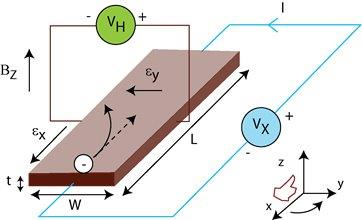
\includegraphics[scale=0.5]{Immagini/12_12/image011.jpg}
\caption{Schema dell'effetto di Hall classico\label{fig:hall_classico}}
\end{figure}
\end{expl}
\begin{figure}[H]
\centering
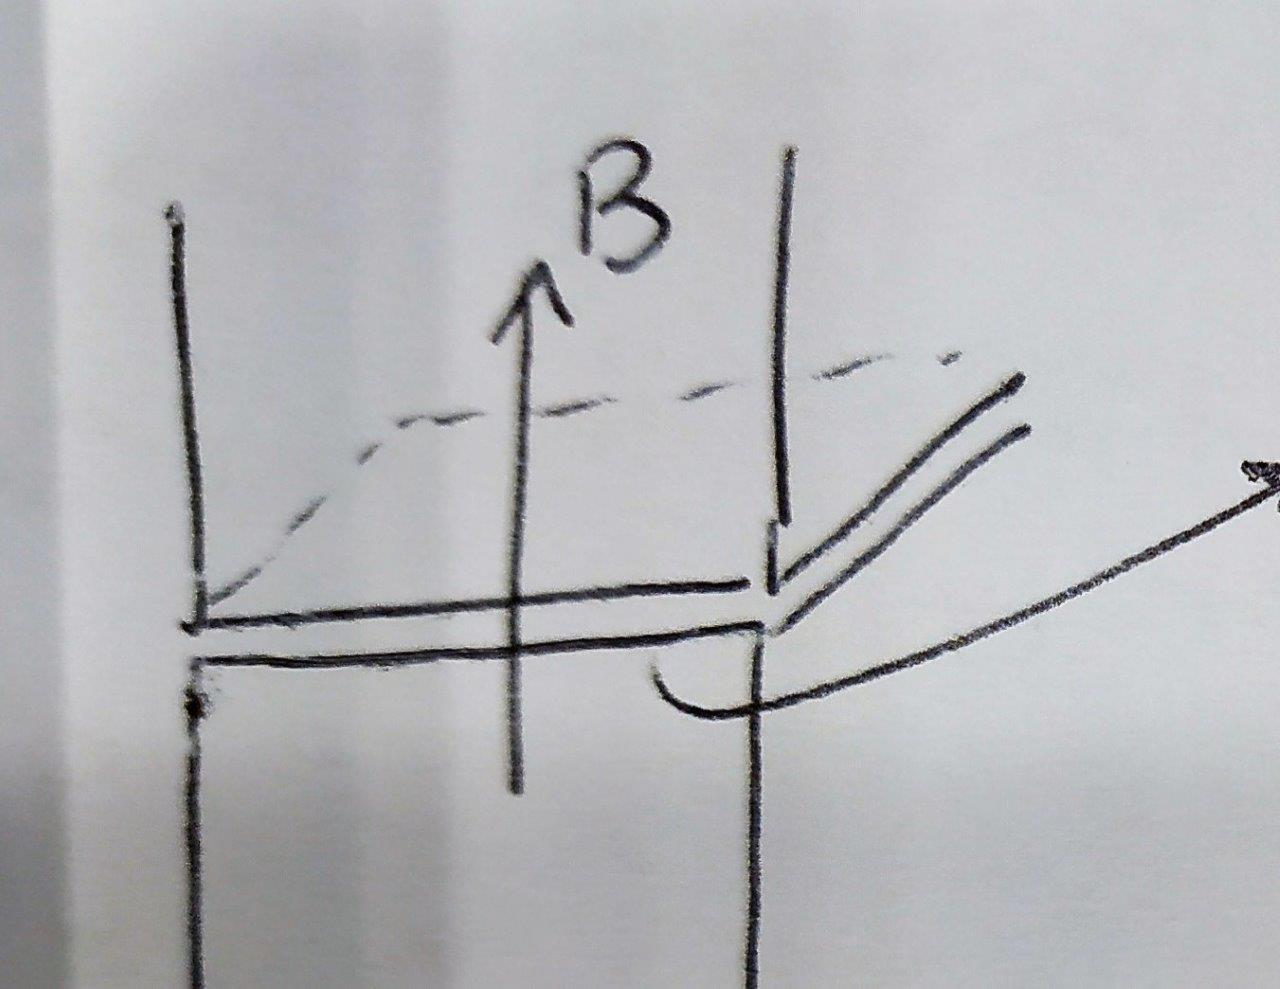
\includegraphics[scale=0.2]{Immagini/12_12/image009.jpg}
\caption{Schema dell'apparato sperimentale per l'effetto di Hall quantistico frazionario}
\end{figure}
Sperimentalmente, consideriamo un interfaccia tra semiconduttori -- per esempio quella tra silicio e strato di ossido in un MOSFET. Introduciamo un campo magnetico $\vec{B}$ perpendicolare all'interfaccia. Gli elettroni sulla superficie del semiconduttore seguono le orbite di ciclotrone, per cui abbiamo i livelli di Landau per le energie, dati da:
\begin{align}
\mathcal{E}_n=\hbar \omega \left(n+\frac{1}{2}\right)\qquad \omega = \frac{eB}{m_e}
\label{eqn:landau_energies}
\end{align}
dove $\omega$ è la pulsazione di ciclotrone.\\
Come osservato in un precedente esercizio %inserire ref specifica
i livelli di Landau sono fortemente degeneri, ossia è possibile avere un gran numero di elettroni alla stessa energia, che si dimostra essere proporzionale all'intensità di $B$. Perciò, all'aumentare del campo magnetico, aumenta sia la \textit{distanza} tra un livello e il successivo (come visibile dalla formula (\ref{eqn:landau_energies})) che il numero di elettroni che possono occupare lo stesso livello.\\
Poiché ad ogni $\mathcal{E}_n$ è associato un gran numero di possibili stati, un grafico della \textit{densità} degli stati in funzione dell'energia è dato da una successione di $\delta$ di Dirac equispaziate, come rappresentato in figura \ref{fig:Landau_ideale}.
\begin{figure}[H]
\centering
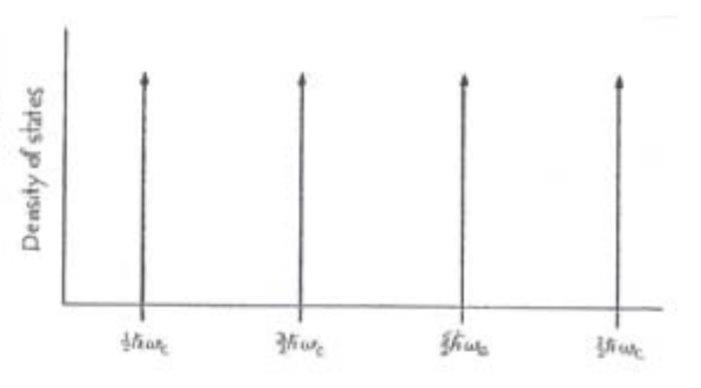
\includegraphics[scale=0.5]{Immagini/12_12/image013.jpg}
\caption{Densità degli stati in funzione dell'energia in un sistema ideale in $d=2$\label{fig:Landau_ideale}}
\end{figure}
Come diretta conseguenza del principio di esclusione di Pauli, $N$ elettroni si disporranno a riempire progressivamente i livelli di Landau partendo da quelli con energia più bassa -- e per temperature $T$ molto basse e $B$ molto alti possiamo considerare trascurabili le eccitazioni termiche tra un livello e un altro, dato che le particelle non hanno abbastanza energia per superare gap sempre più grandi. Risulta perciò ben definita una \textit{energia massima}, detta \textbf{energia di Fermi}, che corrisponde a quella dell'ultimo livello occupato.\\

In realtà, tuttavia, i livelli di Landau non sono ben definiti a causa delle \textit{impurezze} dell'interfaccia. Tali impurezze causano delle \q{buche di potenziale localizzate}, dove gli elettroni possono rimanere intrappolati, come rappresentato in figura \ref{fig:Landau_impurities}.

\begin{figure}[H]
\centering
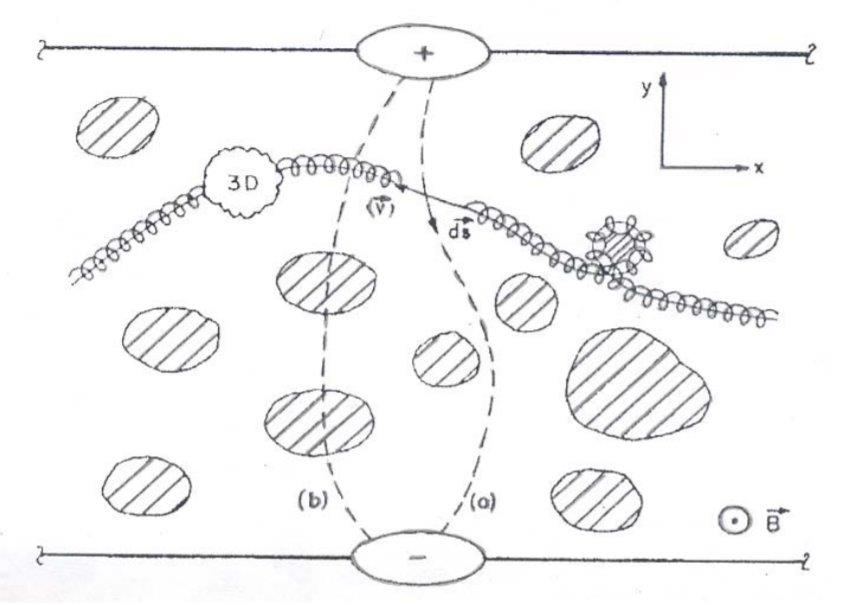
\includegraphics[scale=0.5]{Immagini/12_12/image014.jpg}
\caption{Le impurità nel cristallo sono rappresentate come regioni tratteggiate. Gli elettroni, nel loro moto sulla superficie, possono ritrovarsi in \textit{stati localizzati} attorno alle impurità, con un'energia intermedia tra due livelli di Landau\label{fig:Landau_impurities}}
\end{figure}

Avremo perciò una densità di stati non trascurabile anche ad energie tra $\mathcal{E}_n$ consecutivi. Un grafico più realistico è riportato in figura \ref{fig:Landau_reale}.

\begin{figure}[H]
\centering
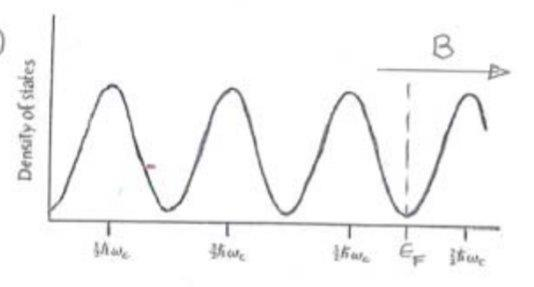
\includegraphics[scale=0.5]{Immagini/12_12/image015.jpg}
\caption{Densità degli stati in funzione dell'energia in un cristallo con impurità\label{fig:Landau_reale}}
\end{figure}

Possiamo ora spiegare l'\textit{effetto di Hall intero}, scoperto nel 1983. Per $T\sim \SI{10}{\kelvin}$ e $B\sim \SI{10}{\tesla}$, si realizza un sistema in cui solo \textit{pochi} livelli di Landau sono riempiti dagli elettroni (ossia si trovano al di sotto dell'energia di Fermi).\\
Detta $n$ la densità di elettroni e $d$ la degenerazione di ogni livello, il numero $\nu$ di livelli riempiti è dato da:
\begin{align*}
n = \nu d
\end{align*}
Per $d$ usiamo la stima già trovata in (\ref{eqn:degenerazione-landau}), per cui arriviamo a:
\begin{align*}
\frac{1}{\nu} = \frac{nh}{eB}
\end{align*}
Si scopre sperimentalmente che $\nu$ assume \textit{valori esattamente interi} non solo per i $B_\nu$ che verificano tale condizione, ma anche per $B$ \q{leggermente diversi}. Questo è l'effetto delle impurità, per cui alcuni elettroni \textit{rimangono intrappolati} in \textit{stati localizzati} ad energie intermedie tra i singoli livelli, e in tal modo \q{stabilizzano} il sistema, facendo sì che vi siano sempre un \textit{numero intero} di livelli riempiti.\\
La conseguenza di ciò è che la \textit{resistività di Hall} $\rho_{xy}$ è quantizzata:
\begin{align*}
\rho_{xy} =\frac{B}{ne} = \nu\frac{h}{e^2}
\end{align*}
In figura \ref{fig:graph-res-hall} è possibile notare come, aumentando progressivamente il campo magnetico, la resistività $\rho_{xy}$, espressa in multipli di $h/e^2$ \q{salga a salti}, rimanendo costante per un certo range di valori di $B$.\\
Allo stesso tempo, la resistività longitudinale $\rho_{xx}$ tende a $0$ durante i singoli \textit{plateau} di $\rho_{xy}$. Ciò è conseguenza del fatto che $\rho_{xx}$ misura la perdita di energia per scattering inelastico degli elettroni, ossia quanta energia perdono \q{per attrito} attraversando la lamina. Ma, se esattamente $\nu$ livelli sono pieni, gli elettroni non hanno posto dove andare, e perciò non perdono energia spostandosi: in effetti, si dimostra che in questi casi anche la conduttanza $\sigma_{xx}$ è nulla.

\begin{figure}[H]
\centering
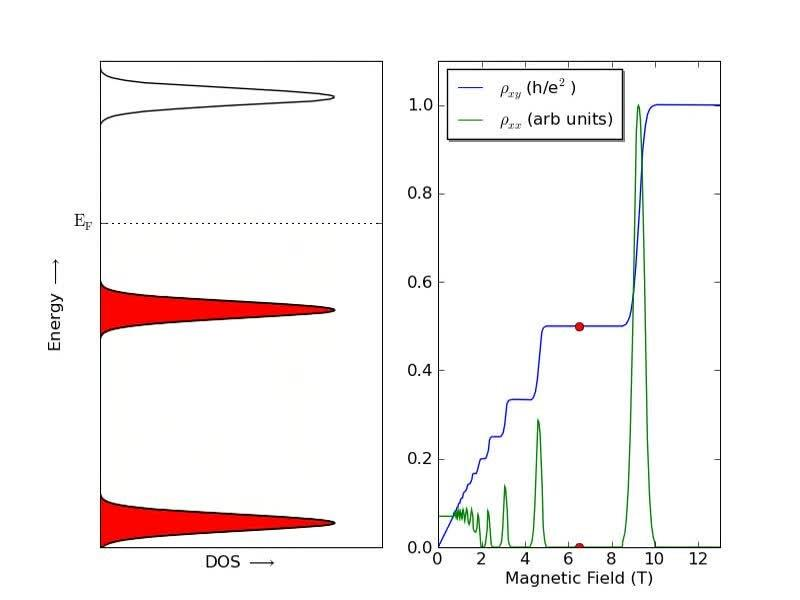
\includegraphics[scale=0.5]{Immagini/12_12/image012.jpg}
\caption{Grafico delle resistività $\rho_{xy}$ e $\rho_{xx}$ in funzione di $B$\label{fig:graph-res-hall}}
\end{figure}

Il punto importante è che l'esistenza in primo luogo dei \textit{plateau} delle resistività è dovuta a imperfezioni del sistema, che hanno effetti di natura \textit{topologica}, nel senso che le funzioni d'onda degli elettroni \q{si arrotolano} attorno alle impurità, rimanendo ivi \textit{localizzate}. Questa situazione rende il sistema molto \textit{stabile}, ed offre possibili applicazioni nella realizzazione di porte logiche per computer quantistici.\\

Poiché tuttavia siamo in $d=2$, si apre la possibilità che rotazioni orarie e antiorarie attorno a impurità \textit{non siano equivalenti}, e che quindi entri in gioco una statistica \textit{di trecce} e non di normali permutazioni. In effetti, questo è proprio quello che succede diminuendo ulteriormente la temperatura a $T\sim 1$K, come fu  scoperto nel 1986.\\

In questo nuovo sistema si trovò che gli elettroni avevano uno stato di energia minimo uniforme, e i livelli eccitati erano costituiti da eccitazioni che obbedivano alla statistica di trecce, con $\theta=2\pi/3$.\\
Se $x,y$ sono le coordinate del piano, definiamo $z=x+iy$. Allora le funzioni d'onda di $N$ di queste eccitazioni sono della forma:
\begin{align*}
\psi(z_1, \dots, z_N) = \prod_{i<j} (z_i - z_j)^{\frac{1}{3}}\prod_{i=1}^N e^{-c|z_i|^2}
\end{align*}
Scambiando in sensio antiorario due particelle, normalmente avremmo $(z_i - z_j) \to e^{i\pi} (z_i -z_j)$, ma ora abbiamo:
\begin{align*}
(z_i-z_j)^{\frac{1}{3}} \to (e^{i\pi}(z_i-z_j))^{\frac{1}{3}} = e^{i\frac{\pi}{3}}(z_i - z_j)^{\frac{1}{3}}
\end{align*}
Analogamente, uno scambio orario sarebbe $(z_i-z_j) \to e^{-i\pi (z_i-z_j)}$, ma qui diviene:
\begin{align*}
(z_i-z_j)^{\frac{1}{3}} \to (e^{-i\pi (z_i - z_j)})^{\frac{1}{3}}= e^{-i\frac{\pi}{3}}(z_i- z_j)^{\frac{1}{3}}
\end{align*}

La differenza appena notata è all'origine di \textit{plateau} della resistività $\rho_{xy}$ anche a \textit{valori frazionari} di $h/e^2$, cosa che non succedeva nel caso dell'effetto di Hall intero.
\end{document}

